\NeedsTeXFormat{LaTeX2e}
\documentclass[twocolumn]{ECMS}
\usepackage{preamble}
% \usepackage[english,russian]{babel}
% \usepackage{multirow}

%% Usage:
%% \documentstyle[..,Xpt,twoside]{IEEEtran}
%% \author{..}
%% \title{..}
%% \maketitle
%% \begin{abstract}...\end{abstract}
%% \begin{keywords}...\end{keywords}
%% ... main text ...
%% \begin{biography}{Author's name}...\end{biography}
%% \end{document}

%\documentstyle[twocolumn,Xpt,twoside]{IEEEtran}

\author{
    \normalsize
    \begin{tabular}{cc}
        Olga Chaganova & Anton Grigoryev \\
        Institute for Information & Institute for Information \\
        Transmission Problems, RAS & Transmission Problems, RAS \\ 
        Bolshoy Karetny per.~19, Moscow, 127051, Russia; & Bolshoy Karetny per.~19, Moscow, 127051, Russia \\
        Moscow Institute of Physics and Technology & E-mail: me@ansgri.com \\
        (National Research University) & \\
        Institutskiy per.~9, Dolgoprudny, 141701, Russia & \\
        E-mail: o.chaganova@visillect.com & \\
        & \\
    \end{tabular}
}


% \title{\textbf{\TODO{PARAMETERIZED NEURAL NETWORK APPROXIMATION OF CLASSICAL IMAGE PROCESSING ALGORITHMS}}}
\title{\textbf{LEARNED PARAMETERIZED CONVOLUTIONAL APPROXIMATION OF IMAGE FILTERS % GRAYSCALE MORPHOLOGICAL DILATION
}}
\begin{document}
\maketitle

% Suppress page numbering 
\thispagestyle{empty}\pagestyle{empty}


%% Do not use the following keywords and abstract environment, use \section instead to get desired layout
%%\begin{keywords}
%%Agent-based modelling; Genetic algorithms
%%\end{keywords}
%%
%%\begin{abstract}
%%Abstract goes here. This is an example of using the ECMS \LaTeX\ class.
%%\end{abstract}

%% Notes about sections: Use star * to avoid numbering of sections

\section*{\textbf{KEYWORDS}}
Convolutional neural networks, grayscale morphology, edge detection, computational efficiency, image processing

\subimport{}{chapters/abstract.tex}
\subimport{}{chapters/intro.tex}
\subimport{}{chapters/theory.tex}
\subimport{}{chapters/evaluation.tex}
\subimport{}{chapters/conclusion.tex}

\section*{\textbf{ACKNOWLEDGMENT}}

This work is partially financially supported by Russian Foundation for Basic Research (project 18-29-26037).
 
\renewcommand{\bibsection}{}
\setlength{\bibhang}{18pt}
\section*{\textbf{REFERENCES}}
\bibliographystyle{ecms}
\bibliography{biblio}

\vskip 24 pt

\mysection{\bf{AUTHOR BIOGRAPHIES}}

\begin{wrapfigure}{l}{0.1\textwidth}
    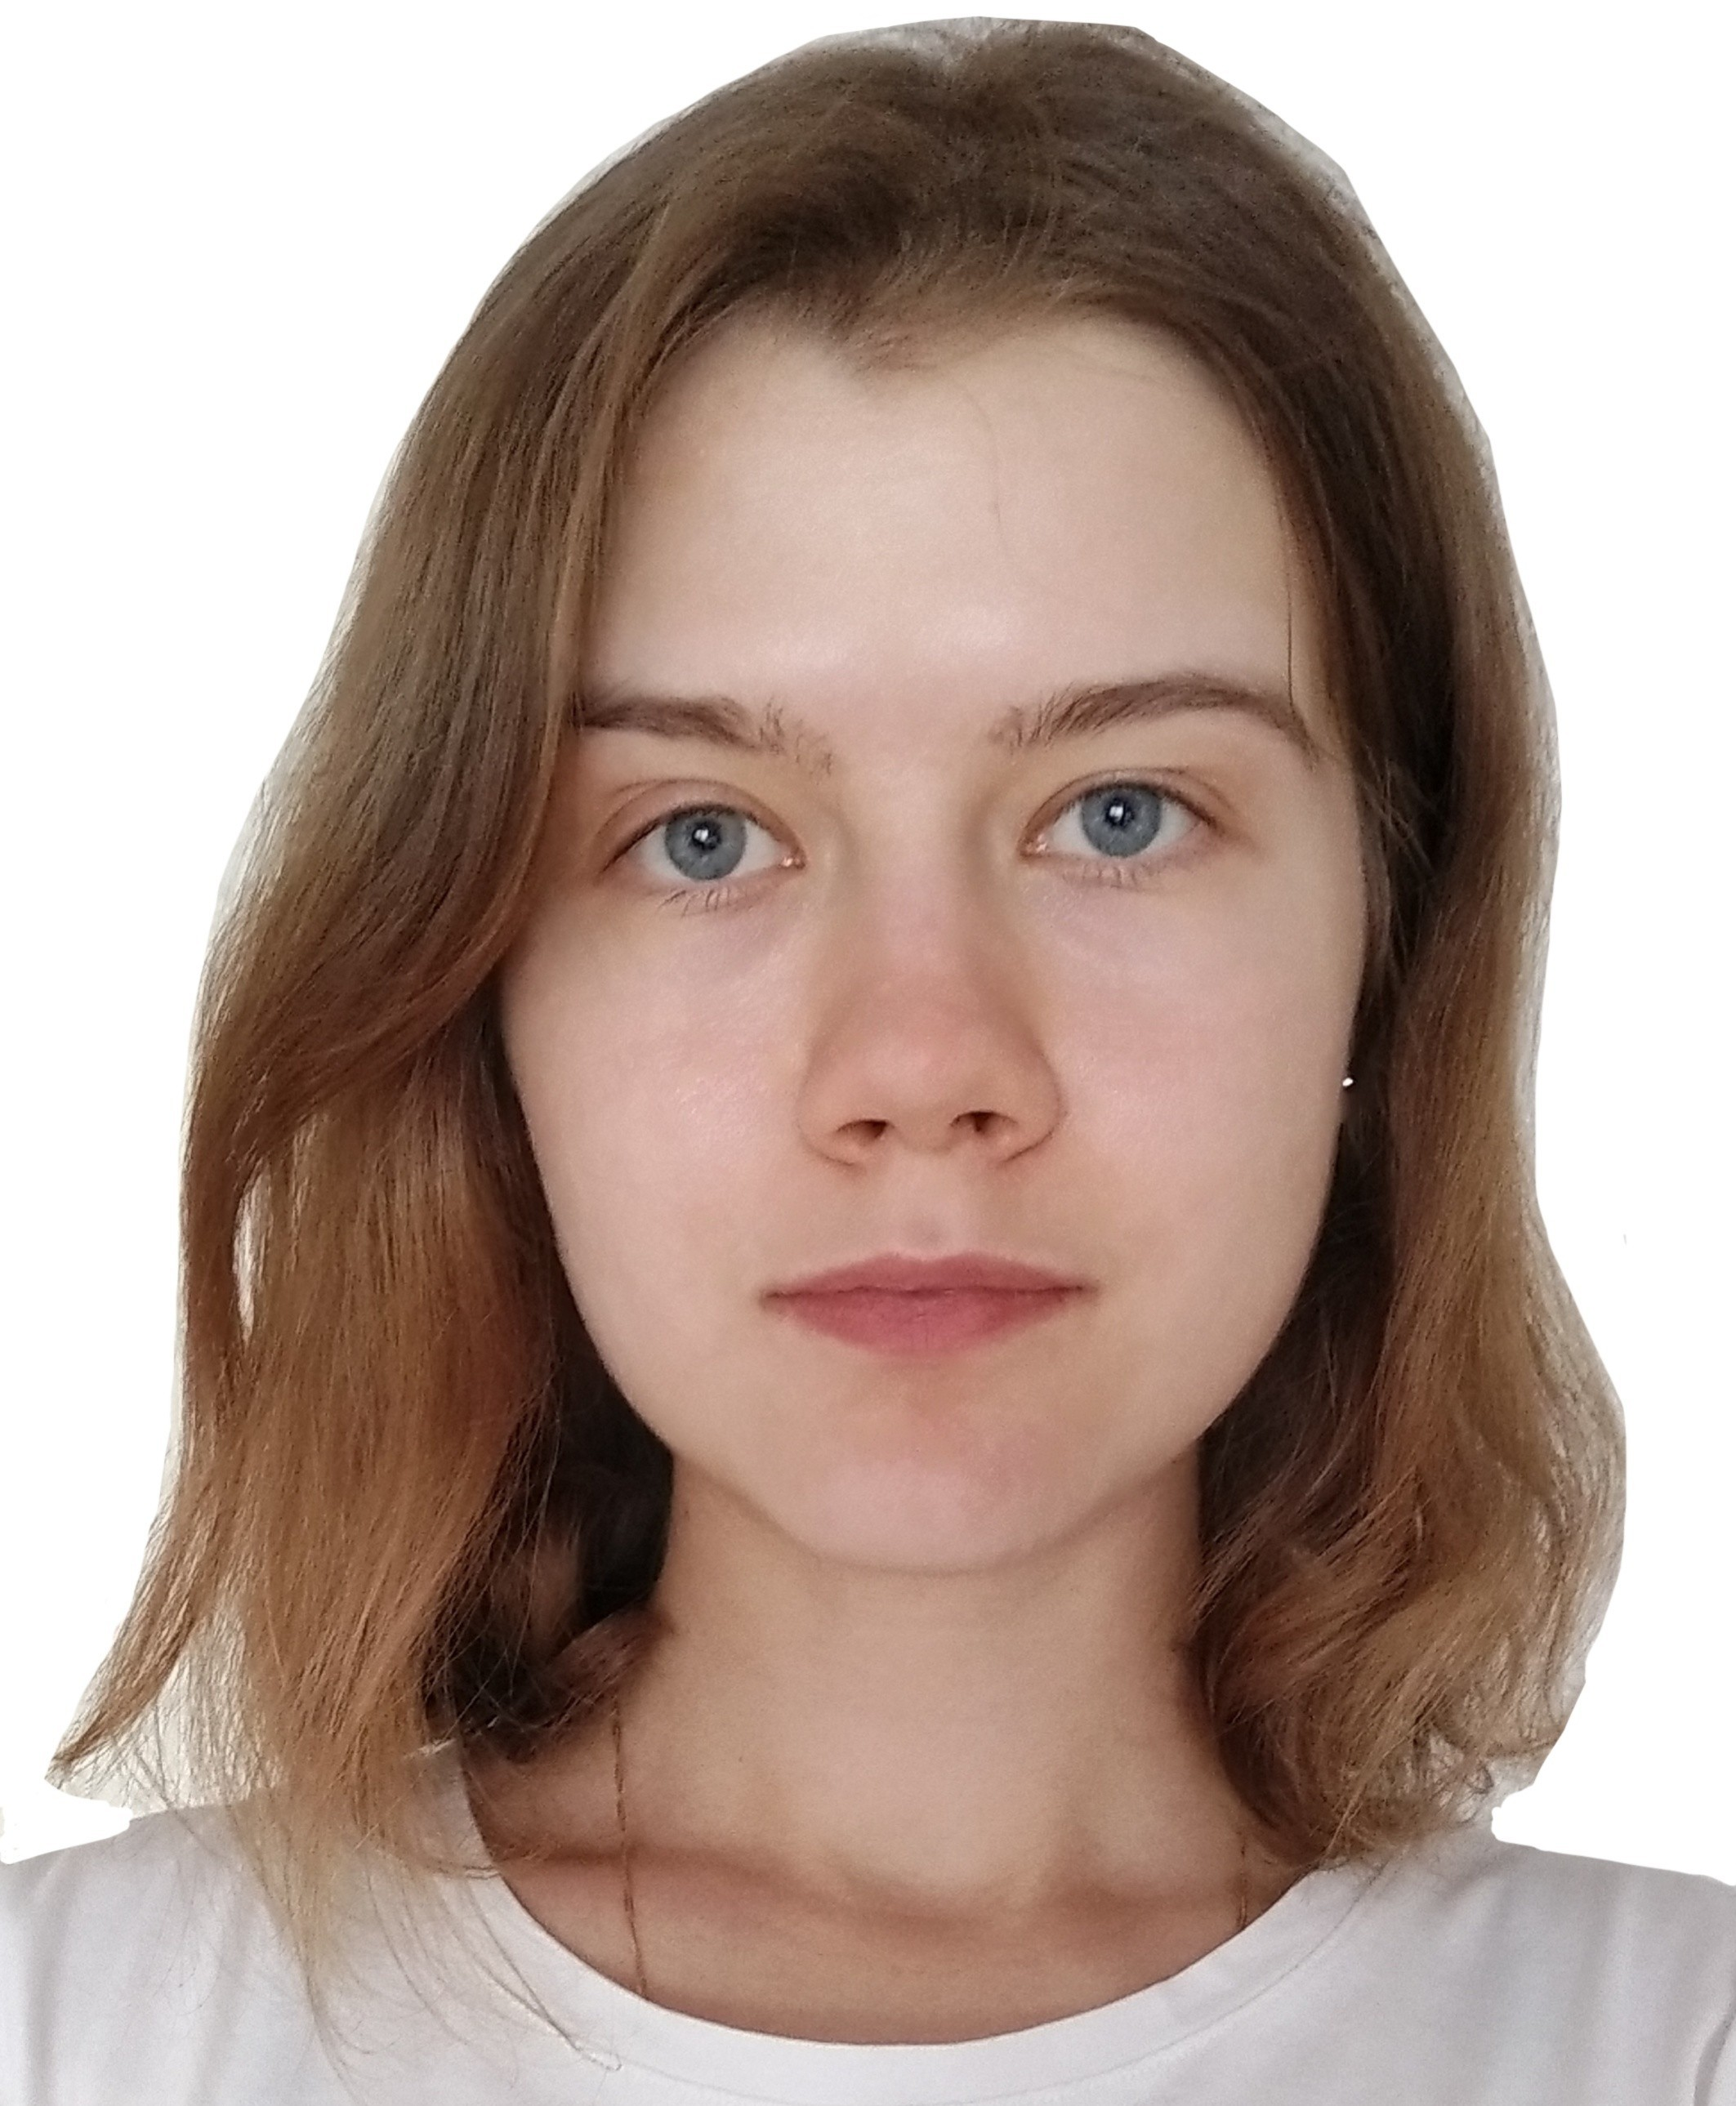
\includegraphics[width=0.145\textwidth]{fig/chaganova.jpg}
\end{wrapfigure}
\noindent \textbf{{\MakeUppercase{Olga Chaganova}}} 
\noindent was born in Orenburg, Russia.
Currently she is a M.Sc. student in Applied Mathematics and Physics at Moscow Institute of Physics and Technology.
Since 2021, she works as a junior research fellow at the Vision Systems Lab of the Institute for Information Transmission Problems.
Her research interests include deep learning and computer vision. 
Her email address is o.chaganova@visillect.com.
\\

\begin{wrapfigure}{l}{0.1\textwidth}
  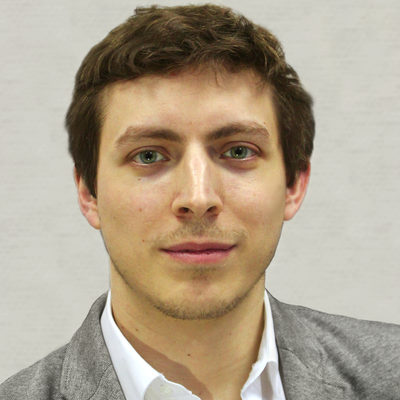
\includegraphics[width=0.14\textwidth]{fig/grigoryev.jpg}
\end{wrapfigure}
\noindent \textbf{{\MakeUppercase{Anton Grigoryev}}} 
\noindent was born in Petropavlovsk-Kamchatskiy, Russia.
Having graduated from Moscow Institute of Physics and Technology, he has been developing industrial computer vision systems with the Vision Systems Lab at the Institute for Information Transmission Problems since 2010.
His research interests are image processing and enhancement methods, autonomous robotics and software architecture.
His e-mail address is me@ansgri.com.
\\




\end{document}